\begin{figure}[tp]
 \centering
 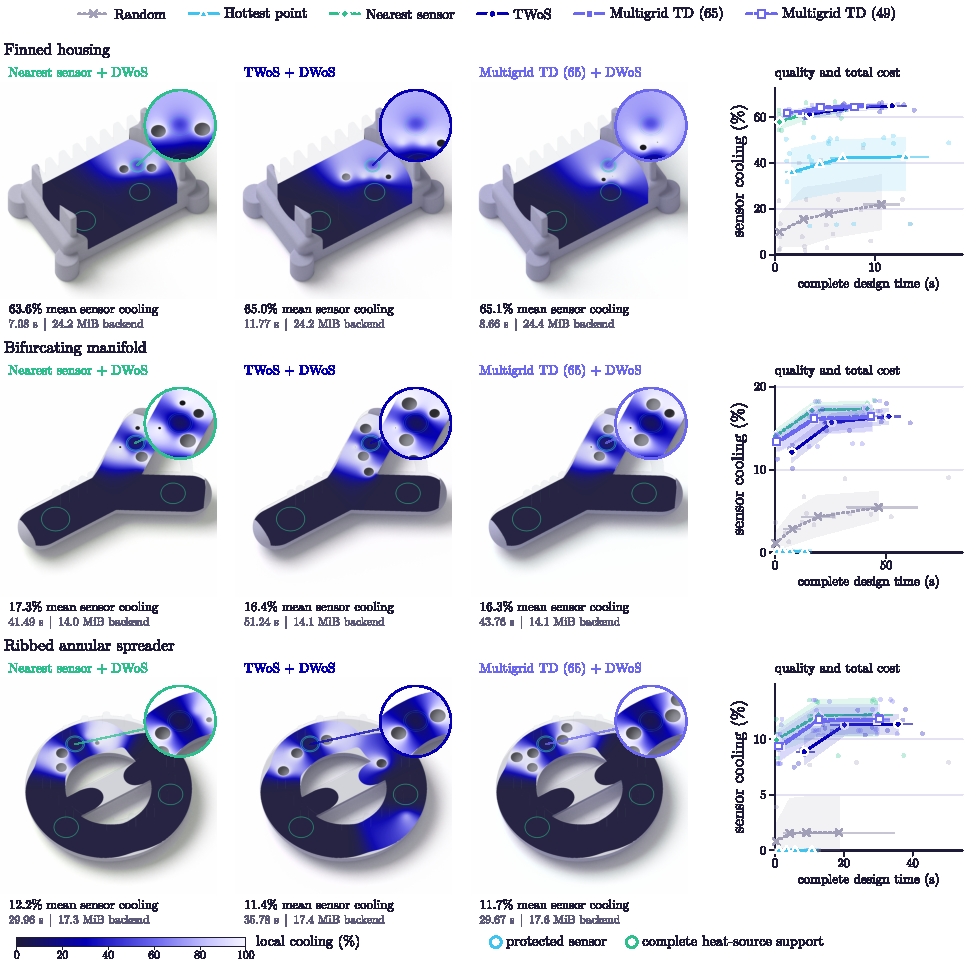
\includegraphics[width=\textwidth]{figures/submission-pipeline.pdf}
 \caption{\textbf{Insertion decisions affect the refined design.}
 Each row fixes the physical domain, protected sensor, heat input, cavity count,
 and exact removed volume. Views show the first predeclared seed after refinement;
 cyan and mint outlines mark the sensor and complete source supports. The
 section color shows local cooling relative to the unperforated temperature,
 from a common multigrid rendering field. It is not the objective's confidence
 interval. Labels and curves summarize five design seeds; faint dots show
 individual runs. Bands are pointwise 95\% bootstrap intervals for mean sensor
 cooling, jointly resampling seeds and independent evaluation blocks;
 horizontal bars resample complete runtime across seeds. Plot ranges adapt
 to each geometry; units and the local-cooling color scale are shared. They do not cover
 numerical bias. Hot and random receive up to sixteen refinement rounds;
 TWoS, both multigrid selectors, and nearest-sensor placement receive eight. Ghost shells show material
 removed only for display; some cavities lie outside the section. Independent evaluation, rendering, and mesh
 generation are excluded from design time.}
 \label{eg:submissionpipeline}\label{fig:submissionpipeline}
\end{figure}
